\chapter{NNUE-Implementierung}

Ziel dieses Kapitels ist es, Architektur und Implementierung der im Rahmen dieser Arbeit entwickelten \ac{NNUE}-Evaluationsfunktion zu erläutern. Es wird anfangs auf die Architekturentscheidungen eingegangen. Danach wird geklärt, wie diese Entscheidungen Einfluss auf die Implementierung des Trainers und auf die Integration in einem Schachcomputer haben.

Kapitel \autoref{chap:HCE} zeigt, wie die herkömmliche Art und Weise der Positions-Evaluation funktioniert. Verbesserungen der \ac{HCE} sind nicht einfach. Jeder neue Aspekt in der Evaluationsfunktion muss sorgfältig ausgewählt werden und anschließend per Hand oder mithilfe von Optimierungsalgorithmen, wie \zb{} \ac{SPSA}, angepasst werden \cite{spall1992multivariate}. Es ist sehr schwierig, eine Evaluation zu bauen, die für alle möglichen Stellungen optimal ist. Zudem spielt der Bias der Entwickler immer eine Rolle. Die \ac{NNUE}-Evaluation ist nicht an solche Limitierungen gebunden und kann auf eine ganz andere Art und Weise entscheiden, welche Faktoren wichtig für die Evaluation einer Schachposition sind. Die Entwicklung der Schachcomputerlandschaft zeigt, dass diese Herangehensweise der \ac{HCE} überlegen ist. Nur in Situationen, in denen es einen klaren Vorteil gibt, ist es sinnvoll \ac{HCE} zu verwenden. Deshalb verwenden die meisten \ac{NNUE}-Schachcomputer einen hybriden Ansatz in der Implementierung. In dieser Arbeit wird eine reine \ac{NNUE}-Evaluation verwendet. Der Grund dafür ist die rudimentäre \ac{HCE} des verwendeten Schachcomputers. Außerdem tritt dieser Fall bei Schachcomputer gegen Schachcomputer selten auf, da der Vorteil meist klein bleibt.

\section{Architektur}

Die in dieser Arbeit verwendete Architektur ist keine Neue. Sie ist die von \citeauthor{YNasu2018} \cite{YNasu2018} vorgeschlagene Architektur, die ebenfalls in der ersten \ac{NNUE}-Version von Stockfish verwendet wurde. Sie eignet sich für diesen Prototyp, da sie alle Elemente der \ac{NNUE}-typischen Architektur enthält und die Grundlage für komplexere Architekturen wie die aktuelle von Stockfish (siehe \autoref{chap:relatedWork}) ist. Kleinere Architekturen, wie anfangs in \autoref{chap:featureSet} mit $768$ Merkmalen, zeigen Verbesserungen über \ac{HCE} in schwächeren Schachcomputern, wie der in dieser Arbeit verwendete. Jedoch nutzen sie nicht das Potenzial von \ac{NNUE} aus und tauschen die Spielstärke gegen eine simplere Implementierung.

Die Architektur, welche in dieser Arbeit verwendet wird, ist in \autoref{fig:own-nn} zu sehen. Die Eingabeschicht stellt den dünn besetzten binären Eingabevektor dar. Für das Laden der Daten wird ein Datenlader von Stockfish verwendet, da die verwendeten Trainingsdaten auch von Stockfish sind. Dieser Datenlader hat als Relikt aus der Shogi-Implementierung ein HalfKP-Feature Set mit $41024$ statt den für Schach nötigen $40960$ Merkmalen \cite{StockfishNNUE}. Das hat aufgrund der spaltenweisen Berechnung des Akkumulators keinen Einfluss auf die Performance.

\begin{figure}
  \centering
  \resizebox{\textwidth}{!}{%
    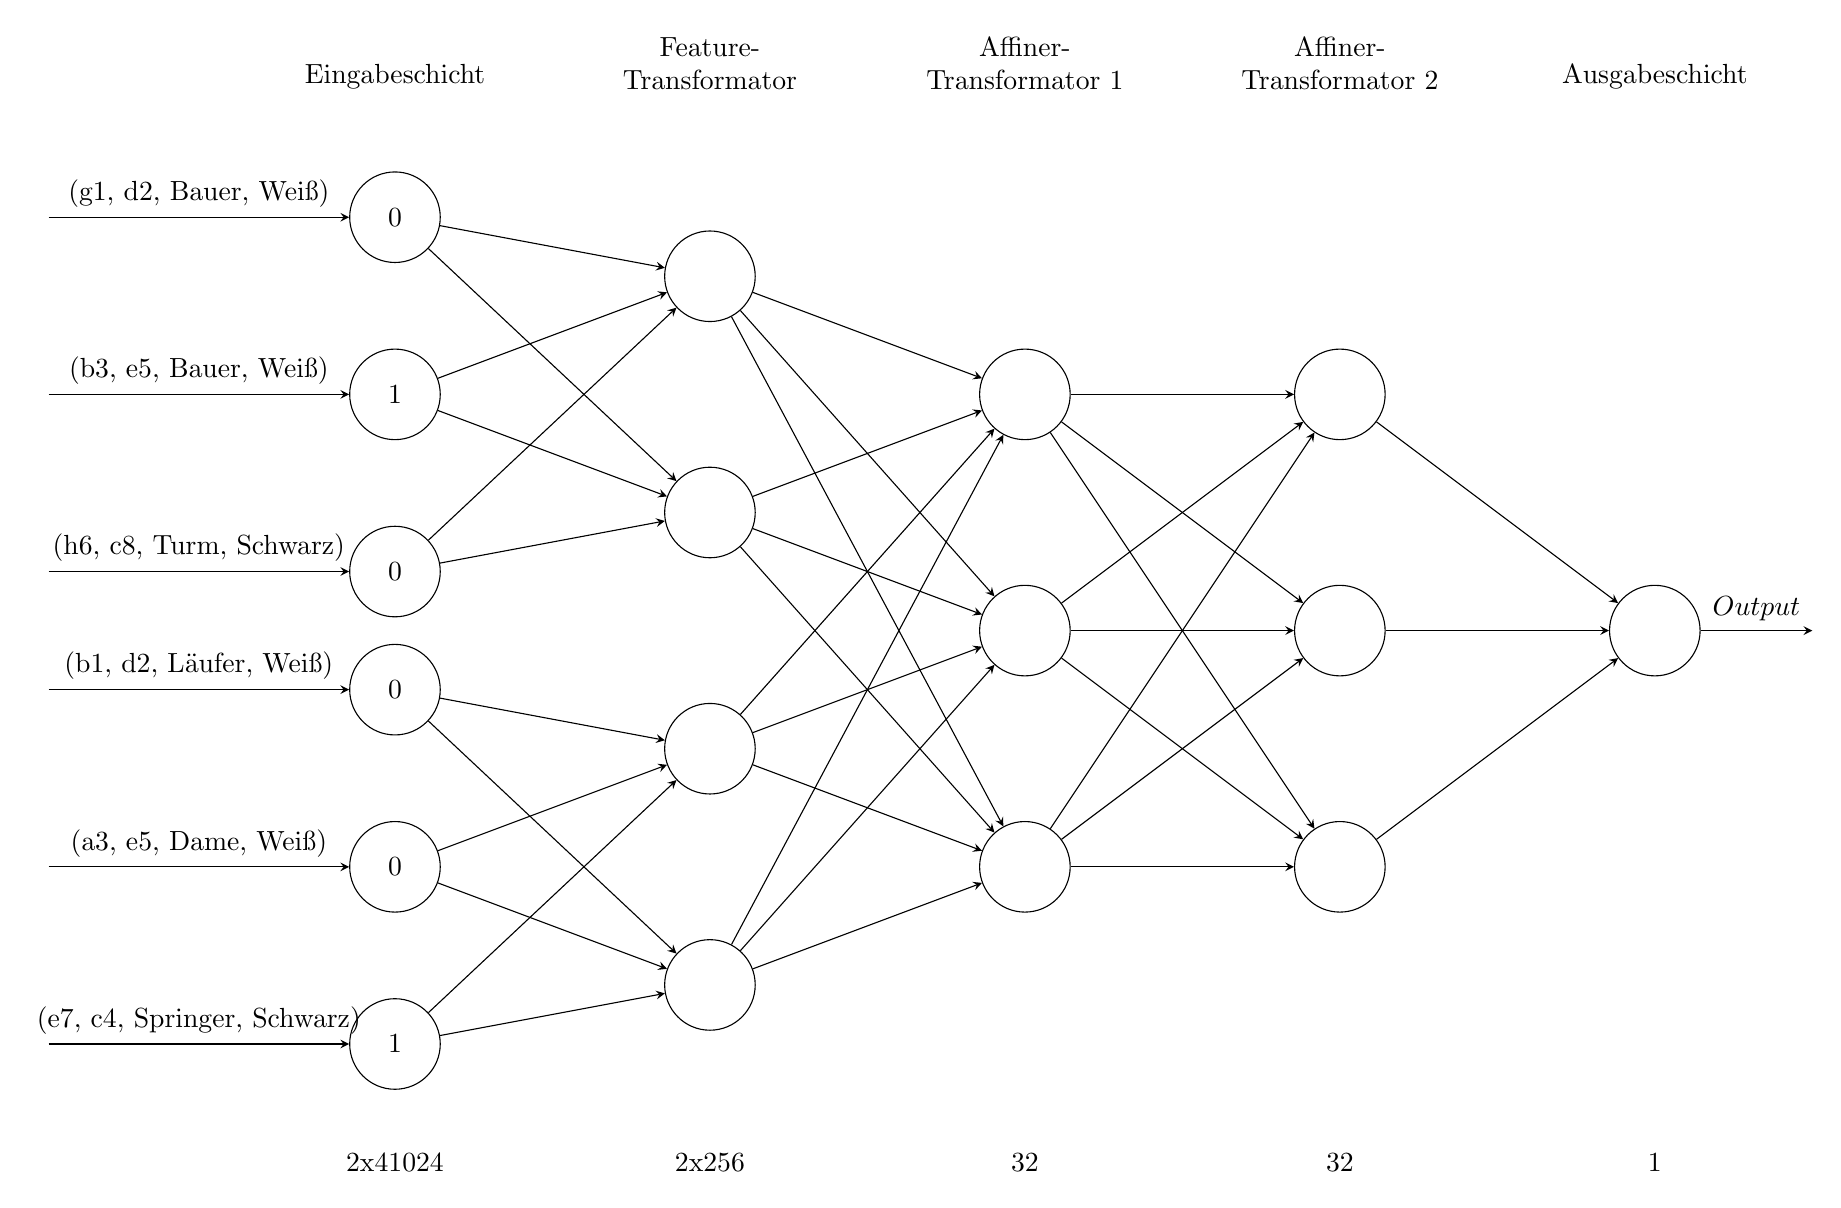
\begin{tikzpicture}[x=2cm, y=1.5cm, >=stealth]
      \tikzstyle{neuron}=[draw,shape=circle,minimum size=1.15cm]
      % draw nerons

      \foreach \m/\l [count=\y] in {0,1,0}
      \node [neuron] (input1-\y) at (0,2.5-\y*1.5) {\m};

      \foreach \m/\l [count=\y] in {0,0,1}
      \node [neuron] (input2-\y) at (0,-1.5-\y*1.5) {\m};

      \foreach \m [count=\y] in {1,2}
      \node [neuron] (inputL11-\m) at (2,2.5-\y*2) {};

      \foreach \m/\l [count=\y] in {1,2}
      \node [neuron] (inputL12-\m) at (2,-1.5-\y*2) {};

      \foreach \m/\l [count=\y] in {1,2,3}
      \node [neuron] (hidden1-\m) at (4,1.5-\y*2) {};

      \foreach \m/\l [count=\y] in {1,2,3}
      \node [neuron] (hidden2-\m) at (6,1.5-\y*2) {};

      \foreach \m [count=\y] in {1}
      \node [neuron] (output-\m) at (8,-1.5-\y) {};

      % draw text  

      \foreach \l [count=\x from 0] in {2x41024, 2x256, 32, 32, 1}
      \node [align=center] at (\x*2,-7) {\l};

      \draw [->] (output-1) -- ++(1,0) node [above, midway] {$Output$};

      \foreach \l [count=\x from 0] in {Eingabeschicht, Feature-\\Transformator, Affiner-\\Transformator 1, Affiner-\\Transformator 2, Ausgabeschicht}
      \node [align=center, above] at (\x*2,2) {\l};
      % draw lines  

      \draw [->] (-2.2,1) node {} -- node [midway,above] {(g1, d2, Bauer, Weiß)} (input1-1);
      \draw [->] (-2.2,-0.5) node {} -- node [midway,above] {(b3, e5, Bauer, Weiß)} (input1-2);
      \draw [->] (-2.2,-2) node {} -- node [midway,above] {(h6, c8, Turm, Schwarz)} (input1-3);

      \draw [->] (-2.2,-3) node {} -- node [midway,above] {(b1, d2, Läufer, Weiß)} (input2-1);
      \draw [->] (-2.2,-4.5) node {} -- node [midway,above] {(a3, e5, Dame, Weiß)} (input2-2);
      \draw [->] (-2.2,-6) node {} -- node [midway,above] {(e7, c4, Springer, Schwarz)} (input2-3);

      \foreach \i in {1,2,3}
      \foreach \j in {1,2}
      \draw [->] (input1-\i) -- (inputL11-\j);

      \foreach \i in {1,2,3}
      \foreach \j in {1,2}
      \draw [->] (input2-\i) -- (inputL12-\j);

      \foreach \i in {1,2}
      \foreach \j in {1,2,3} {
          \draw [->] (inputL11-\i) -- (hidden1-\j);
          \draw [->] (inputL12-\i) -- (hidden1-\j);};

      \foreach \i in {1,2,3}
      \foreach \j in {1,2,3}
      \draw [->] (hidden1-\i) -- (hidden2-\j);

      \foreach \i in {1,2,3}
      \foreach \j in {1}
      \draw [->] (hidden2-\i) -- (output-\j);

    \end{tikzpicture}
  }%
  \caption{Das verwendete \ac{NN} mit einer exemplarischen Eingabe, basierend auf der \autoref{fig:chessboard}. Die Bezeichnung der Schichten ist oberhalb und die Anzahl der dazugehörigen Neuronen unterhalb des Netzes zu sehen. Die Eingabeschicht und die Feature-Transformator-Schicht sind in zwei Teile geteilt, basierend auf den zwei Seiten im Schach (Weiß und Schwarz). Sonst sind die Schichten voll vernetzt. Die Ausgabe des Netzes ist eine Evaluation der Position.}
  \label{fig:own-nn}
\end{figure}

Das \acl{DNN} ist untypisch klein, da die meiste Information in der Feature-Transformator-Schicht enthalten ist \cite{StockfishNNUE}. Die übrigen Schichten müssen klein gehalten werden, da sie nicht wie die Feature-Transformator-Schicht mit inkrementellen Aktualisierungen aktiviert werden. Sie werden immer ganz berechnet werden. Die Ausgabeschicht besitzt lediglich ein Neuron, da es sich hier um ein Regressionsproblem handelt. Die Ausgabe des Neurons spiegelt die Evaluation einer Schachposition wider.

Für die Berechnung einer Evaluation ist theoretisch eine Schicht ausreichend. Das limitiert das Netz jedoch sehr stark in der Form der zu modellierenden Funktion. Deshalb werden hier wie üblich für \acp{DNN} mehrere Schichten verwendet. Die genaue Zusammensetzung der Schichten ist darauf ausgelegt, dass die Neuronen einer Schicht die Größe der verwendeten \ac{SIMD}-Register ganz ausschöpfen \cite{YNasu2018}. Weiter ist es nicht klar, welche Größe sich am besten für den spezifisch verwendeten Schachcomputer eignet. Zur Ermittlung einer optimalen Größe müssen Tests mit verschiedenen Größen durchgeführt werden. Es wird die Größe verwendet, welche bereits Erfolge in anderen Schachcomputern gezeigt hat.
% the reason for choosing an architecture with two hidden layers is based on two things. 1. we dont want a large net to keep processing speed high 2. we use discoveries from other sucessfull engines that also use two hidden layers (e.g. stockfish) 
% theoratically we can use only one layer to approximate a function to convert inputs to an evaluation but thats makes it mutch harder to learn
% because we are looking for regression we use a clipped relu

In \autoref{fig:own-nn} ist die Aktivierungsfunktion nicht zu erkennen. Sie ist ein elementarer Bestandteil dafür, dass die Evaluation der Stellung schnell ist. Deshalb wird die Clipped\ac{ReLU} Transferfunktion verwendet. Sie ist nicht linear und kann schnell berechnet werden. Eine Aktivierung mehrerer Neuronen ist mit \ac{SIMD} gleichzeitig berechenbar. Die Limitierung nach oben ermöglicht die Verwendung von int8 für die Vektoren, die innerhalb des Netzes weitergegeben werden.

\subsection{Feature-Transformator-Schicht}

Die Feature-Transformator-Schicht hat den größten Einfluss auf Geschwindigkeit und Größe \cite{StockfishNNUE}. Das gesamte \ac{NN} hat $10,5$ Millionen trainierbare Parameter. Circa $99,8\%$, also fast alle, sind Teil der Feature-Transformator-Schicht. Das ist untypisch für neuronale Netze. Da aber aufgrund des HalfKP-Feature Sets maximal 30 Merkmale aktiv sein können, ist die tatsächlich verwendete Anzahl an Parametern, pro Zug, deutlich kleiner.

In \autoref{fig:own-nn} ist der Feature-Transformator in zwei Teile geteilt. Einer für Weiß und einer für Schwarz. Je Seite werden 256 Neuronen verwendet. Tatsächlich sind die Gewichte, in dieser Implementierung, für beide Seiten dieselben. Für Weiß werden die Gewichte so wie sie sind verwendet, und für Schwarz wird das Brett um 180 Grad rotiert. Das bedeutet, die schwarzen Figuren werden wie Weiße behandelt und nutzen so die dieselben Gewichte. Eine 180-Grad-Rotation wird wegen des verwendeten Datenladers benutzt.

Eine 180-Grad-Rotation entspricht nicht der Realität, da Schach, im Gegensatz zu Shogi, keine Rotationssymmetrie besitzt. Trotzdem funktioniert es überraschend gut \cite{StockfishNNUE}. Alternativ kann das Brett horizontal gespiegelt werden, um die Symmetrie zu wahren. Eine Illustration warum, wie sich Rotation und Spiegelung erhalten ist in \autoref{fig:orientedChessboards} zu sehen. In der Abbildung ist die orientierte Stellung aus \autoref{fig:chessboard} abgebildet. Sie ist dann nötig, wenn schwarz am Zug ist. Die Farben der Figuren werden invertiert. Das ermöglicht es, die Bewertung für Schwarz aus Sicht von Weiß durchzuführen und so dieselben Gewichte zu verwenden. Diese Orientierung findet während der Generierung der Indizierung der Figuren für die Eingabeschicht statt.

\begin{figure}
  \centering
  \begin{subfigure}{.5\textwidth}
    \centering
    \resizebox{.9\textwidth}{!}{%
      \chessboard[setfen={8/8/6k1/5N2/3p4/8/3K4/8 b}]
    }
    \caption{Um 180-Grad-Rotiertes Schachbrett}
    \label{fig:rotatedChessboard}
  \end{subfigure}%
  \begin{subfigure}{.5\textwidth}
    \centering
    \resizebox{.9\textwidth}{!}{%
      \chessboard[setfen={8/8/1k6/2N5/4p3/8/4K3/8 b}]
    }
    \caption{Horizontal gespiegeltes Schachbrett}
    \label{fig:flippedChessboard}
  \end{subfigure}
  \caption{Beispiele für ein orientiertes Schachbrett. Basierend auf \autoref{fig:chessboard}. Das Schachbrett ist in zwei Orientierungs-Möglichkeiten gezeigt. Die Schachbretter werden für Schwarz ausgerichtet, das ist der Fall, wenn Schwarz am Zug ist. Die Farben sind invertiert. So können die gleichen Gewichte für weiß und Schwarz verwendet werden.}
  \label{fig:orientedChessboards}
\end{figure}

% sparse inputs -> little changes
% max 32 inputs setboolean
% input either 0 or 1
Außerdem ist es für den Akkumulator wichtig, dass bei der Quantisierung ein Quantisierungsschema verwendet wird, welches einen Überlauf verhindert, egal welche Kombination von Merkmalen aktiv ist \cite{StockfishNNUE}.

\subsection{Affine-Transformator-Schichten}

Die Affine-Transformator-Schichten sind voll vernetzte Schichten. Sie werden mit der Clipped\ac{ReLU} Transformation aktiviert und dienen dazu dem Netz mehr Tiefe zugeben, ohne dabei zu groß zu werden. Die zwei hier zugehörigen Schichten haben jeweils 32 Neuronen.

% TODO: hier elaborieren

Aufgrund der Fehler-Akkumulation der Quantisierung kann es passieren, dass größere/mehr Schichten nahe der Ausgabeschicht einen negativen Effekt haben \cite{StockfishNNUE}. Deshalb werden diese Schichten im Vergleich zu der Eingabeschicht sehr klein gehalten.

\section{Training}

Das Training eines \acp{NN} beschreibt den Vorgang, bei welchem die Gewichte des Netzes mithilfe von Backpropagation und Gradientenabstieg angepasst werden. Die Gewichte, werden nach dem Training nicht mehr verändert.
% Nach dem Training werden die Gewichte nicht mehr verändert.

Welche Gewichte gewählt werden, hängt von einigen Faktoren ab. In diesem Kapitel wird auf diese eingegangen. Der Trainingsvorgang lässt sich in zwei Teile teilen. Erstens die Auswahl/Generierung der Eingabedaten, welche die Basis des \acp{NN} sind. Zweitens der Trainer. Er beschreibt das Programm, welches die Daten einliest und die Gewichte anpasst. Der Trainer ist selbst in weitere Teile untergliedert, die Stellschrauben für das Training darstellen.

\subsection{Eingabedaten}
\label{chap:inputdata}

Die Erzeugung der Eingabedaten ist nicht Teil dieser Arbeit. Jedoch ist es wichtig zu wissen, wie die Eingabedaten generiert werden und wie sie in den Trainer geladen werden, um zu verstehen, wie das \ac{NN} lernt. Auf die Implementierung des Stockfish Datenladers wird hier ebenfalls nicht eingegangen, da es nicht relevant für das Verständnis eines \acp{NNUE} ist.

Im Training für diese Arbeit wurden drei verschieden generierte Datensätze verwendet. Diese Datensätze wurden von Stockfish für das Training der neuesten Variante ihres \acp{NNUE} verwendet \cite{StockfishNewestNetJul04}. Die drei Datensätze unterscheiden sich in der Art und Weise, wie sie generiert wurden. Alle Datensätze sind durch Schachcomputer automatisch, mit Spielen gegen sich selbst, generiert. Einer der Datensätze enthält Spieldaten von Stockfish, aus Spielen mit einer festen Suche von $5000$ Knoten pro Zug in Kombination mit dem \ac{UHO}-Eröffnungsbuch \cite{Pohl2021}. Laut Stockfish eignen sich Daten generiert mit \ac{Lc0} generell besser für \acp{NNUE} \cite{StockfishTrainingDataWiki}. Deshalb besteht einer der drei Datensätze aus eine Mischung von verschieden \ac{Lc0} Daten. Trotzdem ist empirisch belegt, dass eine Kombination der Daten zu einem besseren Ergebnis führen. Der dritte Datensatz besteht aus Spieldaten von Stockfish aus der Schachvariante \ac{DFRC}. \ac{DFRC} gibt eine zufällige Startposition der Figuren vor. \emph{Double}, weil beide Seiten unterschiedliche Startpositionen der Figuren haben. Der \ac{DFRC} Datensatz ist für Stockfish interessanter als für diese Arbeit, da Stockfish diesen Modus unterstützt und das mit demselben Netz wie auch herkömmliches Schach. Das ist keine Anforderung für diese Arbeit, da lediglich traditionelles Schach unterstützt ist. Alle Drei Datensätze enthalten insgesamt 72 Milliarden Positionen.

% wenn Eingabedaten mit einer tieferen Suche verwendet werden, sind die Konzepte hinter den Zügen/der Evaluation schwerer zu verstehen und somit auch schwieriger zu lernen.
Es ist nicht klar, welche Daten sich am besten für das Training eines \acp{NNUE} eignen \cite{StockfishNNUE}. Die für diese Arbeit verwendeten Daten haben sich empirisch als geeignet erwiesen. Sind die gewählten Trainingsdaten zu komplex, ist es schwer zu erkennen, welche die Charakteristiken einer guten/schlechten Position sind. Komplexe Daten sind Evaluationen, die mit einer hohen Suchtiefe generiert werden. Ist die Suchtiefe jedoch zu niedrig, ist die Evaluation ungenau und vermittelt möglicherweise falsche Muster.

% ein Problem ist auch, dass die Eingabedaten nicht wirklich den tatsächlichen Anwendungsfall repräsentieren -> das Netzwerk soll die aktuelle Stellung gut bewerten, bekommt aber als Eingabe die Bewertung der Stellung in z. B. 5 Zügen.
Ein weiteres Problem ist es, dass die verwendeten Daten nicht den Anwendungsfall wider Spiegeln. Das Netzwerk soll die aktuelle Stellung so genau wie möglich Evaluieren, die Eingabedaten zeigen jedoch die Evaluationen von Positionen welche \zb{} nur 5000 Knoten tief gesucht wurde.

% die Reihenfolge von den Daten spielt eine Rolle
Ein Netz kann mehrmals trainiert werden. Das ist sinnvoll, wenn dabei verschiedene Eingabedaten verwendet werden. Dabei ist die Reihenfolge der Datensätze von Bedeutung. Es kann besser für das Training sein, wenn zuerst simple Daten und dann komplexere Daten verwendet werden. Verschiedene Testergebnisse dazu sind in \autoref{chap:Ergebnisse} zu sehen. Außerdem kann es sein das ein Trainingslauf, aufgrund der Zufällig initialisierten Gewichte, in einem lokalen Minimum stecken bleibt. Das wird jedoch vernachlässigt, da es deutlich mehr Trainingsläufe bräuchte um diesen Effekt zu verringern.

% normalerweise ist wird pro Epoche das gesamte Datenset verarbeitet, hier ist das nicht der Fall, wir verarbeiten 100M Positionen pro Zug, wichtig ist, dass die Daten nicht sequentiell gelesen werden, deshalb werden zufällige Positionen übersprungen -> würden die Daten gesuffelt sein, wären die Eingabedaten sehr viel größer, da ihr Encoding auf sich wenig ändernden Positionen basiert
% Letztendlich werden alle Positionen gleich oft trainiert, die Verteilung ist jedoch besser zum Lernen.
Eine Epoche ist als 100 Millionen Positionen definiert. Eine Batch, also die Zahl an Positionen, die in einer Iteration verarbeitet werden, beträgt $2^{14}=16.384$. Die Daten werden nicht sequentiell geladen. Sonst würde eine Batch viele ähnliche Stellungen enthalten, da die Daten aufgrund des verwendeten Datenformats, aufgrund von Datenkomprimierung, ähnliche Stellungen sequentiell speichern. Die Daten werden in zufälligen Schritten übersprungen.

% they are already normalized (siehe feature set)
% labeling is easy as the set is automatically generated data with labels (cp score) automatically generated

% grouping the inputdate to a batch size aims to use the time writing to the GPU more efficently (16384)

% there is no great risk of overfitting to the training set because the input data is so large -> generalisation should be strong enogth so that training data acurracy and validation data accuracy cant diverge, and becuase we dont know what the "correct" input looks like any validation data set is usless

Theoretisch gibt es Daten, die \enquote{perfekt} sind, denn Schach ist für Stellungen mit 7 Figuren gelöst. Das heißt, es gibt eine Datenbank, die das eindeutige Ergebnis (-1, 0, 1) für die Position mit perfektem Spiel kennt. Es ist jedoch nicht sinnvoll, diese Informationen für das Training eines \acp{NNUE} zu verwenden. Das Netz ist nicht in der Lage zu verstehen, warum die Stellung gewonnen/verloren ist. Die Konzepte sind oft schwer zu verstehen und der Vorteil wird oft erst in weiter Zukunft realisiert. Außerdem führt die Verwendung dieser Daten zu einem Bias in der Datenbasis, da sie zu einer Übergewichtung von Endspieldaten führen.

% TODO: nicht zufrieden mit dem Titel
\subsection{Trainer}
\label{chap:trainer}

% Trainer means the (pytorch lightning) module that is responsible for training
Der Trainer übernimmt die Anpassung der Gewichte. Er nimmt die Eingabedaten, aktiviert das Netz vorwärts und passt die Gewichte mit Backpropagation an. Der Trainer muss nicht selbständig implementiert werden, Frameworks, wie in diesem Fall PyTorch, vereinfachen die Implementierung \cite{NEURIPS2019_9015}. PyTorch ist ein Python Framework, für das Training von neuronalen Netzen. Es ermöglicht durch vorgefertigte Module die Definition und Training des Netzes auf der GPU.

% descripe training steps:
% 1. initilize network
Zuerst müssen die Schichten des Netzes definiert werden. Die vier Schichten können mit vier Zeilen code definiert werden, wie in \autoref{code:model} zu sehen. Dabei handelt es sich um vier dicht vernetzte lineare Schichten.

\lstinputlisting[language=Python,
  caption={Definition der \ac{NNUE}-Schichten mit PyTorch, wie auf \autoref{fig:own-nn}. Für Schwarz und Weiß werden jeweils dieselben gewichte mittels einer 180-Grad-Rotation verwendet.},
  label=code:model,
  linerange={4-7}]
{\srcloc/model.py}

% repeat following steps for each iteration
% 2. forward activation
Bei der Fehlerrückführung wird zuerst die Vorwärtsaktivierung von der Eingangs- bis zur Ausgabeschicht durchgeführt. Bei diesem \ac{NNUE} wird die Ausgabe der Feature-Transformator-Schicht per Konkatenation, abhängig von der aktiven Seite kombiniert, da die Ausgabe der Ausgabewert die Evaluation aus Sicht der Aktiven Seite darstellen soll und dasselbe Netz für beide Seiten verwendet werden soll. Die Implementierung dazu ist in \autoref{code:forward} zu sehen.

% die Aktivierungsfunktion is eine ClippedReLU
\lstinputlisting[language=Python,
  caption={Die Vorwärtsaktivierung des in \autoref{code:model} definierten Netzes. Die Schichten werden nacheinander, mit der Clipped\ac{ReLU} Transferfunktion, aktiviert. Nach der Feature-Transformator-Schicht werden die beiden Sichtweisen durch Konkatenation kombiniert. Die Eingabedaten werden der Funktion als Parameter gegeben. Welche Seite am Zug ist, wird durch \emph{us} und \emph{them} symbolisiert. Die dünnbesetzten Vektoren \emph{white} und \emph{black} enthalten die Eingabedaten},
  label=code:forward,
  linerange={9-17}]
{\srcloc/model.py}

% 3. evaluate loss either with crossentropy or mse (bouth testet, whats best is in the results chapter)
% convert cp score converted to wdl to reduce gradients -> also decreases the evaluation range -> große Evaluationen sind nicht wichtig -> win more scenario
Nachdem ein Ausgabewert mit dem Netz generiert wurde muss die Genauigkeit dieser Vorhersage bestimmt werden. Dafür wird die Kreuzentropie-Verlustfunktion verwendet. Wird der Fehler auf der \acl{CP} Ausgabe bestimmt, ist der Gradient sehr groß \cite{StockfishNNUE}. Deshalb wird die Ausgabe mit der Sigmoidfunktion zu einer Gewinnwahrscheinlichkeit (0-1) transformiert. Die hier verwendete Kreuzentropie-Verlustfunktion ist von Stockfish übernommen \cite{StockfishNNUE}. Sie leitet relativ zu der Ausgabe des Netzes ab, sodass der Fehler mindestens 0 ist. Im Training gibt es außerdem die Besonderheit, das anhand der Evaluation der Position oder über das Ergebnis der gespielten Partie in der Stellung gelernt werden kann. Welches Verhältnis der zwei Zielwerte optimal ist, lässt sich nicht einfach bestimmen. Es ist möglich, dass die Inklusion Ergebnis basierten Trainings gar nicht hilft. Empirische Tests dazu sind in \autoref{chap:Ergebnisse} zu sehen. Die folgende Implementierung enthält code für dafür. Die Variable \emph{lambda\_} steuert das Verhältnis. Ein kleiner Wert (epsilon) sorgt dafür, um $log(0)$ zu verhindern. Zwei Skalierungswerte sorgen dafür, dass die Ausgabe des Netzes eine passende Form für die Gewinnwahrscheinlichkeit eines Schachspiels darstellt. Die Werte hängen von der Schachcomputer Implementierung und den verwendeten Eingabedaten ab \cite{StockfishNNUE}. Das Folgende \autoref{code:trainingStep}, zeigt die Implementierung eines Training Schritts, der die Eingabedaten bekommt, eine Vorwärtsaktivierung durchführt, den Fehler mit der Kreuzentropie-Verlustfunktion berechnet und den Fehler zurückgibt:

\lstinputlisting[language=Python,
  caption={Die per Parameter übergebenen Eingabedaten werden vorwärts aktiviert. Danach werden die als \ac{CP} vorhandenen Werte Skaliert. Anschließend wird die Entropie und der Fehler für Evaluation und Ergebnis ermittelt, sodass mit \emph{lambda\_} ein Verhältnis der beiden Einflüsse gebildet werden kann. Schlussendlich gibt die Funktion die Abweichung der Vorhersage von der erwarteten Ausgabe zurück},
  label=code:trainingStep,
  linerange={21-38}]
{\srcloc/model.py}

% 4. backpropagation using the Adadelta optimization algorithm
% benefits: no learning rate tuning needed is already implemented in pytorch
Mit der Genauigkeit der Ausgabe des Netzes werden mithilfe von Backpropagation die Gewichte angepasst. In dem Training für diese Arbeit wird das adaptive Lernraten-Modell Adadelta \cite{Zeiler2012} verwendet. Adadelta übernimmt die Anpassung der Lernrate und ist bereits von PyTorch implementieren, kann somit sehr einfach, wie \autoref{code:adadelta} zeigt, in den Trainer eingebunden werden.

\lstinputlisting[language=Python,
  caption={Deklaration des Optimierungsalgorithmus in PyTorch. Das PyTorch Modul \emph{optim} bietet verschiedene Optimierungsalgorithmen an. Es wird, die Instanziierung der Adadelta Klasse, dargestellt. Die \emph{paramters} ist eine Liste der Parameter der in \autoref{code:model} deklarierten Schichten. Die Lernrate beträgt standardmäßig 1 und wird, durch den Algorithmus, dynamisch angepasst},
  label=code:adadelta,
  linerange={43-43}]
{\srcloc/model.py}

\section{Integration in einen Schachcomputer}
\label{chap:integration}

Folgendes Kapitel beschreibt die Implementierung eines \acp{NNUE} in einen Schachcomputer mit dem Fokus auf \ac{SIMD}-Operationen. Die verwendete Implementierung ist eine auf den Schachcomputer angepasste Version der Stockfish-Implementierung bevor Stockfish zu HalfKAv2 und Buckets gewechselt ist \cite{StockfishRepo}. Da es sich um die gleiche Architektur handelt, bietet es sich an, diese Implementierung zu verwenden.

\subsection{Quantisierungsschema}

Eine Quantisierung ist nötig, um CPU-Optimierungen zu ermöglichen. Die als Float trainierten Gewichte und Bias werden bei der Konvertierung des Netzes von einem \emph{.ckpt} zu einer proprietären binären \emph{.nnue}-Datei konvertiert. Alternativ kann die Konvertierung beim Einlesen der Gewichte und Bias in den Schachcomputer stattfinden. Das hat den kleinen Nachteil, dass die Netzwerkdatei etwas mehr Speicherkapazität benötigt. Das hier verwendete Quantisierungsschema ist dem von Stockfish nachempfunden \cite{StockfishNNUE}. Es ist daran ausgerichtet, die kleinstmöglichen Integer-Typen zu verwenden. Aufgrund der Clipped\ac{ReLU}-Transferfunktion sind die Gewichte bereits sehr klein. Deshalb werden sie mit bestimmten Faktoren multipliziert, um eine hohe Präzision beizubehalten. In \autoref{table:netQuantization} sind die Faktoren und Datentypen für jede Schicht angegeben. Die zwei linearen Schichten unterscheiden sich nicht und werden deshalb in der Auflistung zusammengefasst. Der Ausgabetyp der Schichten ist ebenfalls aufgelistet. Er ist nicht Teil der Quantisierung der Gewichte und Bias, aber wichtig für das Verständnis. Die Werte müssen so gewählt werden, dass keine mögliche Kombination von aktiven Merkmalen den Akkumulator überlaufen lässt \cite{StockfishNNUE}.

\begin{table}[ht]
  \caption{Skalierfaktor und Datentypen für Gewichte und Bias des \acp{NNUE} sowie Ausgabetyp der Schichten. Basierend auf Werten der Stockfish \ac{NNUE} Implementierung \cite{StockfishNNUE}}
  \label{table:netQuantization}
  \renewcommand{\arraystretch}{1.2}
  \centering
  \sffamily
  \begin{footnotesize}
    \resizebox{\textwidth}{!}{%
      \begin{tabular}{l l l l l l}
        \toprule
        \textbf{Schicht}              & \textbf{Gewicht Skalierfaktor} & \textbf{Gewichtstyp} & \textbf{Bias Skalierfaktor} & \textbf{Biastyp} & \textbf{Ausgabetyp} \\
        \midrule
        \emph{Feature-Transformator}  & 127                            & int16                & 127                         & int16            & int8                \\
        \emph{Affine-Transformatoren} & 64                             & int8                 & 8128                        & int32            & int8                \\
        \emph{Ausgabeschicht}         & \textasciitilde75,59           & int8                 & 9600                        & int32            & int32               \\
        \bottomrule
      \end{tabular}
    }%
  \end{footnotesize}
  \rmfamily
\end{table}

Für die Aktivierung der Schichten ändert sich der Bereich der Clipped \ac{ReLU} von 0 bis 1 zu 0 bis 127. Dadurch ist der Ausgabetyp aller Schichten, die innerhalb des Netzes sind int8. Der Gewichtstyp der Feature-Transformator muss int16 sein, weil er sonst bei der Akkumulation der HalfKP Features überlaufen kann. Das Problem stellt sich bei den Affine-Transformatoren nicht, da durch \ac{SIMD}-Instruktionen bei der Berechnung des Matrixprodukts der Datentyp automatisch auf int32 angepasst wird. Ein Problem, das hier auftreten kann, ist das Überlaufen der int8-Werte. Deshalb werden sie vor der Multiplikation in beide Richtungen durch $127/64$ begrenzt. Der Bias in den Affine-Transformatoren und der Ausgabeschicht ist hoch, da wir sie mit den int32-Werten der Matrixprodukte addieren und maximale Präzision beibehalten. Die Ausgabeschicht besitzt einen noch höheren Bias-Skalierfaktor, weil die Ausgabe der \ac{NNUE}-Evaluationsfunktion der \ac{HCE} gleichen soll (für hybride Evaluation). Das ist auch wünschenswert für reine \ac{NNUE}-Implementierungen, um eine Vergleichbarkeit der Evaluation verschiedener Schachcomputer/Versionen zu wahren. Der Gewicht-Skalierfaktor der Ausgabeschicht fällt aus der Reihe, da er nicht ganzzahlig ist. Das liegt daran, dass er sich an dem Bias-Skalierfaktor und dem Aktivierungsbereich (127) anpasst, also $9600/127~=75,59$.
% warum ist der Bias-Faktor so hoch? - erklären

\subsection{Feature-Transformator}


\subsection{Affiner-Transformator}
% der Transformator transformiert und der Akkumulator akkumuliert und gibt weiter